\documentclass[twocolumn,10pt]{article}
\title{Identifying Slope of a Line}
\setlength{\columnsep}{20pt} 
\usepackage{amsmath,hyperref,cancel,graphicx}
 
 \def\shrinkfactor{0.55}
 \usepackage[margin=1.5cm]{geometry}
\usepackage[usenames,dvipsnames]{color}
 
 \newcommand{\blue}[1]{{\color{Blue}#1}} 
 \newcommand{\purple}[1]{{\color{Purple}#1}} 
 \newcommand{\red}[1]{{\color{Red}#1}} 
 \newcommand{\green}[1]{{\color{Green}#1}} 
 \newcommand{\gray}[1]{{\color{Gray}#1}} 
  \newcommand{\pink}[1]{{\color{Magenta}#1}}   


\begin{document}
\maketitle



\section{\href{https://www.khanacademy.org/devadmin/content/items/x36bf4ab2}{x36bf4ab2}}

\noindent
Dominique from �Dominique's Pizza� wanted to know how much electricity it takes to bake $1$ pizza. She checked her electricity meter three times in one day. Each time she also recorded the number of pizzas baked until then.  
  
**Assuming the relationship has a constant rate of change, find the exact value of this rate of change using the following table:**  
  

Pizzas baked | Electricity Meter (in $\text{kWh}$*)
:-:|:-:|:-:|
$8$ | $11,\!563$
$23$ | $11,\!581$
$48$ | $11,\!611$  
*$\text{kWh}$ is a measurement unit of energy


\paragraph{Ans} It takes [[? input-number 1]] $\text{kWh}$ to bake $1$ pizza.  1.2

\paragraph{Hint 1}The first row tells us that when $\red{8\text{ pizzas}}$ were baked, the meter was showing $\red{11,\!563\text{ kWh}}$.  
The third row tells us that when $\blue{48\text{ pizzas}}$ were baked, the meter was showing $\blue{11,\!611\text{ kWh}}$. 
  
$\quad\blue{48}-\red{8}=40$    
  
$\quad\blue{11,\!611}-\red{11,\!563}=48$  
  
Therefore, it took $48\text{ kWh}$ to bake $40$ pizzas. Now let's find how much $\text{kWh}$ it takes to bake $1$ pizza.

\paragraph{Hint 2}
\begin{align}
\dfrac{48}{40}&=\dfrac{\cancel{8}\cdot6}{\cancel{8}\cdot5}\\
&=\dfrac{6}{5}\\
&=1\dfrac{1}{5}\\
&=1.2\end{align}

\paragraph{Hint 3}**It takes $1.2\text{ kWh}$ to bake $1$ pizza.**
  
Note that what we did was like finding the slope of a line that passes through the points $(\red{8}, \red{11,\!563})$ and $(\blue{48}, \blue{11,\!611})$, where the $x$-axis represents the number of pizzas baked and the $y$-axis represents the electricity meter.



\medskip
\noindent
\textbf{Tags:} {\footnotesize CC.8.F.B.4, SB.8.1.F.2.CR.2, Slope of a line.1}\\
\textbf{Version:} c6715972.. 2013-10-14
\smallskip\hrule





\section{\href{https://www.khanacademy.org/devadmin/content/items/x4e3f10ba}{x4e3f10ba}}

\noindent
Joshua�s grandmother has an exotic snake that grows the same amount every day. The first time Joshua saw the snake it was $2$ feet long. The last time was $15$ months later and the snake was $8$ feet long.  
  
**What is the rate of change of the snake�s length?**

\paragraph{Ans} The snake grows [[? input-number 1]] feet per month.  0.4

\paragraph{Hint 1}The first time Joshua saw the snake it was $2$ feet long, and $15$ months later, it was $8$ feet long. Therefore, the change in time is $15$ months, and the change in length is:  
  
$\quad8-2=6$ feet  
  
Now let's find the number of feet the snake grows in exactly $1$ month.

\paragraph{Hint 2}\begin{align*}\quad\dfrac{6}{15}&=\dfrac{\cancel{3}\cdot2}{\cancel{3}\cdot5}\\
&=\dfrac{2}{5}\end{align*}

\paragraph{Hint 3}**The snake grows $\frac{2}{5}$ feet per month.**  
  
Note that what we did was like finding the slope of a line that passes through the points $(0,2)$ and $(15, 8)$ ,where the $x$-axis represents the time in months from today, and the $y$-axis represents the length of the snake.



\medskip
\noindent
\textbf{Tags:} {\footnotesize CC.8.F.B.4, SB.8.1.F.2.CR.2, Slope of a line.1}\\
\textbf{Version:} 2924dd50.. 2013-10-14
\smallskip\hrule





\section{\href{https://www.khanacademy.org/devadmin/content/items/x84a31073}{x84a31073}}

\noindent
The table below describes the price of a train ticket according to the number of stops traveled.  
  
**Assuming the relationship between number of stops and price has a constant rate of change, find the value of this rate of change.**  
  
$\text{\#}$ of Stops | Price ($\$$)
:-:|:-:|:-:|
$7$ | $40.60$
$15$| $87$
$21$ | $121.80$  


\paragraph{Ans} The price of the ticket increases by $\$$[[? input-number 1]] per stop.  5.8

\paragraph{Hint 1}The first row tells us that a ticket for traveling $\red{7\text{ stops}}$ costs $\red{\$40.60}$.  
The second row tells us that a ticket for traveling $\blue{15\text{ stops}}$ costs $\blue{\$87}$.  
  
$\quad\blue{15}-\red{7}=8$    
  
$\quad\blue{87}-\red{40.60}=\$46.40$  
  
Therefore, an increase of $8$ stops increases the price by $\$46.40$. Now let's find the increase in price for an increase of $1$ stop.

\paragraph{Hint 2}
\begin{align}\dfrac{46.40}{8}&=\dfrac{10\cdot46.40}{10\cdot8}\\
&=\dfrac{464}{80}\\
&=\dfrac{\cancel{16}\cdot29}{\cancel{16}\cdot5}\\
&=\dfrac{29}{5}\\
&=\$5.80\end{align}.

\paragraph{Hint 3}**The price of the ticket increases by $\$5.80$ per stop.**
  
Note that what we did was like finding the slope of a line that passes through the points $(\red{7}, \red{40.6})$ and $(\blue{15}, \blue{87})$, where the $x$-axis represents the number of stops and the $y$-axis represents the price.



\medskip
\noindent
\textbf{Tags:} {\footnotesize CC.8.F.B.4, SB.8.1.F.2.CR.2, Slope of a line.1}\\
\textbf{Version:} 6e777cab.. 2013-10-14
\smallskip\hrule





\section{\href{https://www.khanacademy.org/devadmin/content/items/x9bf130ee}{x9bf130ee}}

\noindent
Dominic from �Dominic's Pizza� wanted to know how much electricity it takes to bake $1$ pizza. He checked his electricity meter at the beginning of the day and two more times that day. Each time he also recorded the number of pizzas baked until then.  
  
**Assuming the relationship has a constant rate of change, find the exact value of this rate of change using the following table:**  
  

Pizzas baked | Electricity Meter (in $\text{kWh}$*)
:-:|:-:|:-:|
$0$ | $23,\!100$
$15$ | $23,\!110$
$27$ | $23,\!118$  
*$\text{kWh}$ is a measurement unit of energy


\paragraph{Ans} It takes [[? input-number 1]] $\text{kWh}$ to bake $1$ pizza.  0.6666666666666666

\paragraph{Hint 1}The second row tells us that when $\red{15\text{ pizzas}}$ were baked, the meter was showing $\red{23,\!110\text{ kWh}}$.  
The third row tells us that when $\blue{27\text{ pizzas}}$ were baked, the meter was showing $\blue{23,\!118\text{ kWh}}$. 
  
$\quad\blue{27}-\red{15}=12$    
  
$\quad\blue{23,\!118}-\red{23,\!110}=8$  
  
Therefore, it took $8\text{ kWh}$ to bake $12$ pizzas. Now let's find how much $\text{kWh}$ it takes to bake $1$ pizza.

\paragraph{Hint 2}
\begin{align}\dfrac{8}{12}&=\dfrac{\cancel{4}\cdot2}{\cancel{4}\cdot3}\\
&=\dfrac{2}{3}\end{align}

\paragraph{Hint 3}**It takes $\frac{2}{3}\text{kWh}$ to bake $1$ pizza.**
  
Note that what we did was like finding the slope of a line that passes through the points $(\red{15}, \red{23,\!110})$ and $(\blue{27}, \blue{23,\!118})$, where the $x$-axis represents the number of pizzas baked and the $y$-axis represents the electricity meter.



\medskip
\noindent
\textbf{Tags:} {\footnotesize CC.8.F.B.4, SB.8.1.F.2.CR.2, Slope of a line.1}\\
\textbf{Version:} ce0fa92e.. 2013-10-14
\smallskip\hrule





\section{\href{https://www.khanacademy.org/devadmin/content/items/xc6e4d9c8}{xc6e4d9c8}}

\noindent
Jane's grandson has an exotic snake that grows the same amount every day. Today the snake is $22$ feet long. The last time Jane saw the snake before today was $7$ months ago, when it was $12$ feet long.  
  
**What is the rate of change of the snake�s length?**

\paragraph{Ans} The snake grows [[? input-number 1]] feet per month.  1.4285714285714286

\paragraph{Hint 1}$7$ months ago, the snake was $12$ feet long, and today it's $22$ feet long. Therefore, the change in time is $7$ months, and the change in length is:  
  
$\quad22-12=10$ feet  
  
Now let's find the number of feet the snake grows in exactly $1$ month.

\paragraph{Hint 2}$\quad\dfrac{10}{7}=1\dfrac{3}{7}$

\paragraph{Hint 3}**The snake grows $1\!\frac{3}{7}$ feet per month.**  
  
Note that what we did was like finding the slope of a line that passes through the points $(-7,12)$ and $(0, 22)$ ,where the $x$-axis represents the time in months from today (therefore $7$ months *ago* are considered $-7$), and the $y$-axis represents the length of the snake.



\medskip
\noindent
\textbf{Tags:} {\footnotesize CC.8.F.B.4, SB.8.1.F.2.CR.2, Slope of a line.1}\\
\textbf{Version:} 6364e761.. 2013-10-14
\smallskip\hrule





\section{\href{https://www.khanacademy.org/devadmin/content/items/xccc16e2f}{xccc16e2f}}

\noindent
The table below describes the price of a train ticket according to the number of stops traveled.  
  
**Assuming the relationship between number of stops and price has a constant rate of change, find the value of this rate of change.**  
  
$\text{\#}$ of Stops | Price ($\$$)
:-:|:-:|:-:|
$6$ | $35$
$14 $| $77$
$22$ | $119$  


\paragraph{Ans} The price of the ticket increases by $\$$[[? input-number 1]] per stop.  5.25

\paragraph{Hint 1}The first row tells us that a ticket for traveling $\red{6\text{ stops}}$ costs $\red{\$35}$.  
The second row tells us that a ticket for traveling $\blue{14\text{ stops}}$ costs $\blue{\$77}$.  
  
$\quad\blue{14}-\red{6}=8$    
  
$\quad\blue{77}-\red{35}=\$42$  
  
Therefore, an increase of $8$ stops increases the price by $\$42$. Now let's find the increase in price for an increase of $1$ stop.

\paragraph{Hint 2}
\begin{align*}\dfrac{42}{8}&=\dfrac{\cancel{2}\cdot21}{\cancel{2}\cdot4}\\
&=\dfrac{21}{4}\\
&=5\dfrac{1}{4}\\
&=\$5.25\end{align*}.

\paragraph{Hint 3}**The price of the ticket increases by $\$5.25$ per stop.**
  
Note that what we did was like finding the slope of a line that passes through the points $(\red{6}, \red{35})$ and $(\blue{14}, \blue{77})$, where the $x$-axis represents the number of stops and the $y$-axis represents the price.



\medskip
\noindent
\textbf{Tags:} {\footnotesize CC.8.F.B.4, SB.8.1.F.2.CR.2, Slope of a line.1}\\
\textbf{Version:} 9f61255f.. 2013-10-14
\smallskip\hrule





\section{\href{https://www.khanacademy.org/devadmin/content/items/xda8887e6}{xda8887e6}}

\noindent
Anne wanted to know just how efficient is her car's fuel consumption. When her fuel tank had $30$ gallons of fuel she checked the car mileage and it was $1263$ miles. When her fuel tank had $19$ gallons of fuel, the mileage was $1560$ miles.
  
**Assuming the fuel consumption is constant, find its rate of change.**

\paragraph{Ans} Anne's car can drive [[? input-number 1]]  $\text{MPS}$ (miles per gallon).  27

\paragraph{Hint 1}When the amount of fuel was $\red{30\text{ gallons}}$, the mileage was $\red{1263\text{ miles}}$.  
When the amount of fuel was $\blue{19\text{ gallons}}$, the mileage was $\blue{1560\text{ miles}}$.  
  
$\quad\blue{1560}-\red{1263}=297$  
  
So the change in distance is $693$ miles. In order to find the amount of fuel consumed, we need to subtract the opposite values, since the fuel meter tell us how much we *have* and not how much we *use*:  

$\quad\red{30}-\blue{19}=11$  
  
Therefore, the car consumed $11$ gallons of fuel while driving $297$ miles. Now let's find the number of miles it takes to consume exactly $1$ gallon.

\paragraph{Hint 2}$\quad\dfrac{297}{11}=27$

\paragraph{Hint 3}**Anne's car can drive $27\text{ MPS}$ (miles per gallon).**  
  
Note that what we did was like finding the *absolute value* of the slope of a line that passes through the points $(\red{30}, \red{1263})$ and $(\blue{19}, \blue{1560})$, where the $x$-axis represents the fuel meter and the $y$-axis represents mileage.



\medskip
\noindent
\textbf{Tags:} {\footnotesize CC.8.F.B.4, SB.8.1.F.2.CR.2, Slope of a line.1}\\
\textbf{Version:} bb2d4210.. 2013-10-14
\smallskip\hrule





\section{\href{https://www.khanacademy.org/devadmin/content/items/xf79b4711}{xf79b4711}}

\noindent
Elijah wanted to know just how efficient is his car's fuel consumption. When his fuel tank had $45$ gallons of fuel he checked the car mileage and it was $930$ miles. When his fuel tank had $24$ gallons of fuel, the mileage was $1623$ miles.
  
**Assuming the fuel consumption is constant, find its rate of change.**


\paragraph{Ans} Elijah's car can drive [[? input-number 1]] $\text{MPS}$ (miles per gallon).  33

\paragraph{Hint 1}When the amount of fuel was $\red{45\text{ gallons}}$, the mileage was $\red{930\text{ miles}}$.  
When the amount of fuel was $\blue{24\text{ gallons}}$, the mileage was $\blue{1623\text{ miles}}$.  
  
$\quad\blue{1623}-\red{930}=693$  
  
So the change in distance is $693$ miles. In order to find the amount of fuel consumed, we need to subtract the opposite values, since the fuel meter tell us how much we *have* and not how much we *use*:  

$\quad\red{45}-\blue{24}=21$  
  
Therefore, the car consumed $21$ gallons of fuel while driving $693$ miles. Now let's find the number of miles it takes to consume exactly $1$ gallon.

\paragraph{Hint 2}$\quad\dfrac{693}{21}=33$

\paragraph{Hint 3}**Elijah's car can drive $33\text{ MPS}$ (miles per gallon).**  
  
Note that what we did was like finding the *absolute value* of the slope of a line that passes through the points $(\red{45}, \red{930})$ and $(\blue{24}, \blue{1623})$, where the $x$-axis represents the fuel meter and the $y$-axis represents mileage.



\medskip
\noindent
\textbf{Tags:} {\footnotesize CC.8.F.B.4, SB.8.1.F.2.CR.2, Slope of a line.1}\\
\textbf{Version:} ee2f0eab.. 2013-10-14
\smallskip\hrule





\section{\href{https://www.khanacademy.org/devadmin/content/items/x394b867e}{x394b867e}}

\noindent
**Determine which function corresponds to the following graph by finding the rate of change of the graph.**
  

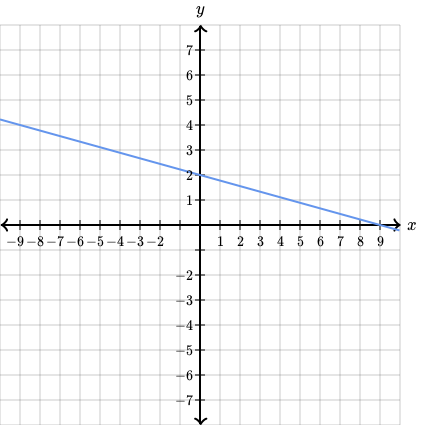
\includegraphics[scale=\shrinkfactor]{figures/61dbf4e2b952dfe6759074d49f6b0f4f6d9f2564.png}

\paragraph{Ans} 

\fbox{ $y=2-\frac{2}{9}x$

}

 $y=2+\frac{2}{9}x$

$y=2-\frac{9}{2}x$

$y=2+\frac{9}{2}x$



\paragraph{Hint 1}Let's find the rate of change of the graph, which is also what we call the *slope* of the graph. We need the exact coordinates of two points the graph passes through, so let's find two points whose values are integers. There are several points like this. We will use $(\red{-9},\red{4})$ and $(\pink{0},\pink{2})$.  
  

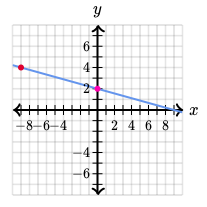
\includegraphics[scale=\shrinkfactor]{figures/3d24a6acea488b6bce2e1425babe02a277549931.png}

\paragraph{Hint 2}The formula of the slope of the graph is **rise over run**, or in other words: (change in $y$)$/$(change in $x$).  
  
\begin{align}\dfrac{\pink{2}-\red{4}}{\pink{0}-(\red{-9})}&=\dfrac{-2}{9}\\
&=-\dfrac{2}{9}\end{align}  
  
Therefore, the rate of change is $-\frac{2}{9}$.

\paragraph{Hint 3}The only function that has the correct rate of change  is:  
$\quad y=2-\dfrac{2}{9}x$  
Therefore, this is the correct function.



\medskip
\noindent
\textbf{Tags:} {\footnotesize CC.8.F.B.4, SB.8.1.F.2.CR.1, Slope of a line.2}\\
\textbf{Version:} 3a58040a.. 2013-10-14
\smallskip\hrule





\section{\href{https://www.khanacademy.org/devadmin/content/items/x4f06de3c}{x4f06de3c}}

\noindent
Paprika the baker likes her bread spicy. For every $6$ grams of table salt she uses, she adds $21$ grams of chili.
  
**Assuming the relationship is *not* proportional, which function can represent the relationship between the amount of table salt in grams, $\text{T}$, and the amount of chili in grams, $\text{C}$?**

\paragraph{Ans} 

\fbox{ $\text{C}=21+\frac{7}{2}\text{T}$

}

 $\text{C}=\frac{7}{2}\text{T}$

$\text{C}=\frac{6}{21}\text{T}$

$\text{C}=6+\frac{2}{7}\text{T}$



\paragraph{Hint 1}We know that for every $6$ grams of table salt she uses, Paprika adds $21$ grams of chili. So how many grams of chili will she add to $1$ gram of table salt?

\paragraph{Hint 2}
\begin{align}\dfrac{21}{6}&=\dfrac{\cancel{3}\cdot7}{\cancel{3}\cdot2}\\
&=\dfrac{7}{2}\end{align}  
  
The rate of change is $\frac{7}{2}$.  
  
There are *two* functions with this rate of change:  
$\quad \text{C}=\dfrac{7}{2}\text{T}$  
and  
$\quad \text{C}=21+\dfrac{7}{2}\text{T}$  
  
How do we decide which is the correct function?

\paragraph{Hint 3}Remember that we are told the relationship is *not proportional*. Since the first equation represents a proportional relationship, we must rule it out.

\paragraph{Hint 4}The only function with the correct rate of change that does not represent a proportional relationship is:  
$\quad\text{C}=21+\dfrac{7}{2}\text{T}$  
Therefore, this is the correct function.



\medskip
\noindent
\textbf{Tags:} {\footnotesize CC.8.F.B.4, SB.8.1.F.2.CR.1, Slope of a line.2}\\
\textbf{Version:} 5ecb3552.. 2013-10-14
\smallskip\hrule





\section{\href{https://www.khanacademy.org/devadmin/content/items/x645810e2}{x645810e2}}

\noindent
"Yak" travel agency came out with a special offer for Mountain Everest - pay as you climb!  
The table below describes the relationship between the altitude of the climb and the price to pay to get there.  
  
**Assuming the rate of change is constant, which function can represent the price paid for climbing, $\text{P}$, as a function of the altitude in meters, $\text{A}$?**  
  
Altitude (meters) | Price ($\$$)
:-:|:-:|:-:|
$5364$  (South Base Camp) | $300$
$7436$ | $559$
$8848$ (the summit!)| $735.50$

\paragraph{Ans} 

$\text{P}=300+8\text{A}$

$\text{P}=735\frac{1}{2}-\frac{1}{8}\text{A}$

\fbox{ $\text{P}=\frac{1}{8}\text{A}-370\frac{1}{2}$

}

 $\text{P}=5362-8\text{A}$



\paragraph{Hint 1}The first row tells us that to get to an altitude of $\red{5364\text{ meters}}$, the price is $\red{\$300}$.  
The second row tells us that to get to an altitude of $\blue{7436\text{ meters}}$, the price is $\blue{\$559}$.  
  
$\quad\blue{7436}-\red{5364}=2072$    
  
$\quad\blue{559}-\red{300}=259$  
  
Therefore, an increase of $2072$ meters in altitude increases the price by $\$259$. Now let's find the increase in price for an increase of $1$ meter in altitude.

\paragraph{Hint 2}\begin{align*}\dfrac{259}{2072}
&=\dfrac{\cancel{259}}{\cancel{259}\cdot8}\\
&=\dfrac{1}{8}\end{align*}  
  
So the rate of change is $\frac{1}{8}$.  
Note that what we did was like finding the slope of the line that passes through the points $(\red{5364}\text{ , }\red{300})$ and $(\blue{7436}\text{ , }\blue{559})$.

\paragraph{Hint 3}The only function with the above rate of change is:  
$\quad\text{P}=\dfrac{1}{8}\text{A}-370\dfrac{1}{2}$  
Therefore, this is the correct function.



\medskip
\noindent
\textbf{Tags:} {\footnotesize CC.8.F.B.4, SB.8.1.F.2.CR.1, Slope of a line.2}\\
\textbf{Version:} f0fe9517.. 2013-10-14
\smallskip\hrule





\section{\href{https://www.khanacademy.org/devadmin/content/items/x6b4b74a2}{x6b4b74a2}}

\noindent
Archimedes is draining his bathtub. Every $2$ minutes that pass, $7$ gallons of water are drained.  
  
**Which function can represent the number of gallons of water in the tub, $\text{W}$, as a function of the minutes that have passed, $\text{T}$?**

\paragraph{Ans} 

$\text{W}=\frac{2}{7}\text{T}$

$\text{W}=\frac{2}{7}\text{T}+20$

\fbox{ $\text{W}=50-\frac{7}{2}\text{T}$

}

 $\text{W}=100+\frac{7}{2}\text{T}$



\paragraph{Hint 1}We know that every $2$ minutes that pass, $7$ gallons of water are drained. So how many gallons of water are drained in $1$ minute?

\paragraph{Hint 2}$\frac{7}{2}$ gallons of water are drained in $1$ minute. Is this the rate of change of the relationship?

\paragraph{Hint 3}$\frac{7}{2}$ gallons is the amount that is *drained*, which means the actual amount of water in the tub  *decreases* as time increases. Therefore, the correct rate of change is $-\frac{7}{2}$.

\paragraph{Hint 4}**The only function with this rate of change is:  
$\quad\text{W}=50-\dfrac{7}{2}\text{T}$  
Therefore, this is the correct function.**  
  
Note that the initial term of the function is $50$, which means that at the beginning of the draining (when $\text{T}=0$) there were $50$ gallons of water in the tub.



\medskip
\noindent
\textbf{Tags:} {\footnotesize CC.8.F.B.4, SB.8.1.F.2.CR.1, Slope of a line.2}\\
\textbf{Version:} 237ddebe.. 2013-10-14
\smallskip\hrule





\section{\href{https://www.khanacademy.org/devadmin/content/items/x6e7b81bf}{x6e7b81bf}}

\noindent
Archimedes is draining his bathtub. Every $6$ minutes that pass, $33$ gallons of water are drained.  
  
**Which function can represent the number of gallons of water in the tub, $\text{W}$, as a function of the minutes that have passed, $\text{T}$?**

\paragraph{Ans} 

$\text{W}=\frac{33}{6}\text{T}$

$\text{W}=\frac{2}{11}\text{T}+27$

\fbox{ $\text{W}=62-\frac{11}{2}\text{T}$

}

 $\text{W}=47-\frac{2}{11}\text{T}$



\paragraph{Hint 1}We know that every $6$ minutes that pass, $33$ gallons of water are drained. So how many gallons of water are drained in $1$ minute?

\paragraph{Hint 2}\begin{align*}\dfrac{33}{6}&=\dfrac{\cancel{3}\cdot11}{\cancel{3}\cdot2}\\
&=\dfrac{11}{2}\end{align*}  
  
$\frac{11}{2}$ gallons of water are drained in $1$ minute. Is this the rate of change of the relationship?

\paragraph{Hint 3}$\frac{11}{2}$ gallons is the amount that is *drained*, which means the actual amount of water in the tub  *decreases* as time increases. Therefore, the correct rate of change is $-\frac{11}{2}$.

\paragraph{Hint 4}**The only function with this rate of change is:  
$\quad\text{W}=62-\dfrac{11}{2}\text{T}$  
Therefore, this is the correct function.**  
  
Note that the initial term of the function is $62$, which means that at the beginning of the draining (when $\text{T}=0$) there were $62$ gallons of water in the tub.



\medskip
\noindent
\textbf{Tags:} {\footnotesize CC.8.F.B.4, SB.8.1.F.2.CR.1, Slope of a line.2}\\
\textbf{Version:} be725829.. 2013-10-14
\smallskip\hrule





\section{\href{https://www.khanacademy.org/devadmin/content/items/x75022488}{x75022488}}

\noindent
The table below describes the relationship between $\text{A}$, the altitude above sea level (in meters), and $\text{T}$, the temperature corresponding to that altitude (in Celsius degrees).  
This relationship has a constant rate of change when the altitude is between sea level and $11,\!000$ meters.$^*$  
  
**Which function can represent the relationship when the altitude is between $0$ and $11,\!000$ meters above sea level?**  
  
Altitude (meters) | Temperature ($^\circ\text{C}$)
:-:|:-:|:-:|
$1000$ | $8\frac{1}{2}$
$3000$ | $-4\frac{1}{2}$
$8000$ | $-37$ 
  
$*$The relationship also has a constant rate of change when the altitude is between $20,\!000$ meters above sea level and $32,\!000$ meters above sea level, but the constant rates are different for each range of altitudes.

\paragraph{Ans} 

\fbox{ $\text{T}=15-\frac{13}{2000}\text{A}$

}

 $\text{T}=\frac{2000}{13}\text{A}$

$\text{T}=\frac{13}{2000}\text{A}+1$

$\text{T}=\frac{2000}{13}\text{A}-1000$



\paragraph{Hint 1}The first row tells us that at an altitude of $\red{1000\text{ meters}}$, the temperature is $\red{8\frac{1}{2}^\circ\text{C}}$.  
The second row tells us that at an altitude of $\blue{3000\text{ meters}}$, the temperature is $\blue{-4\frac{1}{2}^\circ\text{C}}$.  
  
$\quad\blue{3000}-\red{1000}=2000$    
  
$\quad\blue{-4\frac{1}{2}}-\red{8\frac{1}{2}}=-13$  
  
Therefore, an increase of $2000$ meters in altitude *decreases* the temperature by $13^\circ\text{C}$. Now let's find the change in temperature for an increase of $1$ meter in altitude.

\paragraph{Hint 2}$\quad\dfrac{-13}{2000}=-\dfrac{13}{2000}$  
  
So the rate of change is $-\frac{13}{2000}$.  
Note that what we did was like finding the slope of the line that passes through the points $(\red{1000}\text{ , }\red{8\frac{1}{2}})$ and $(\blue{3000}\text{ , }\blue{-4\frac{1}{2}})$.

\paragraph{Hint 3}The only function with the above rate of change is:  
$\quad\text{T}=15-\dfrac{13}{2000}\text{A}$  
Therefore, this is the correct function.



\medskip
\noindent
\textbf{Tags:} {\footnotesize CC.8.F.B.4, SB.8.1.F.2.CR.1, Slope of a line.2}\\
\textbf{Version:} 3b5319ca.. 2013-10-14
\smallskip\hrule





\section{\href{https://www.khanacademy.org/devadmin/content/items/xa2a5f315}{xa2a5f315}}

\noindent
The table below describes the relationship between $\text{A}$, the altitude above sea level (in meters), and $\text{T}$, the temperature corresponding to that altitude (in Celsius degrees).  
This relationship has a constant rate of change when the altitude is between $20,\!000$ meters above sea level and $32,\!000$ meters above sea level.$^*$  
  
**Which function can represent the relationship when the altitude is between $20,\!000$ and $32,\!000$ meters above sea level?**  
  
Altitude (meters) | Temperature ($^\circ\text{C}$)
:-:|:-:|:-:|
$20,\!000$ | $-56\frac{1}{2}$
$27,\!000$ | $-49\frac{1}{2}$
$32,\!000$ | $-44\frac{1}{2}$   
  
$*$The relationship also has a constant rate of change when the altitude is between sea level and $11,\!000$ meters above sea level, but the constant rates are different for each range of altitudes

\paragraph{Ans} 

\fbox{ $\text{T}=\frac{1}{1000}\text{A}-76\frac{1}{2}$

}

 $\text{T}=-\frac{1}{1000}\text{A}-36\frac{1}{2}$

$\text{T}=1000\text{A}-36\frac{1}{2}$

$\text{T}=-\frac{1}{1000}\text{A}-56\frac{1}{2}$



\paragraph{Hint 1}The first row tells us that at an altitude of $\red{20,\!000\text{ meters}}$, the temperature is $\red{-56\frac{1}{2}^\circ\text{C}}$.  
The second row tells us that at an altitude of $\blue{27,\!000\text{ meters}}$, the temperature is $\blue{-49\frac{1}{2}^\circ\text{C}}$.  
  
$\quad\blue{27,\!000}-\red{20,\!000}=7000$    
  
$\quad\blue{-49\frac{1}{2}}-(\red{-56\frac{1}{2}})=-49\frac{1}{2}+56\frac{1}{2}=7$  
  
Therefore, an increase of $7000$ meters in altitude increases the temperature by $7^\circ\text{C}$. Now let's find the increase in temperature for an increase of $1$ meter in altitude.

\paragraph{Hint 2}\begin{align*}\dfrac{7}{7000}&=\dfrac{\cancel{7}}{\cancel{7}\cdot1000}\\
&=\dfrac{1}{1000}\end{align*}  
  
So the rate of change is $\frac{1}{1000}$.  
Note that what we did was like finding the slope of the line that passes through the points $(\red{20,\!000}\text{ , }\red{-56\frac{1}{2}})$ and $(\blue{27,\!000}\text{ , }\blue{-49\frac{1}{2}})$.

\paragraph{Hint 3}The only function with the above rate of change is:  
$\quad\text{T}=\dfrac{1}{1000}\text{A}-76\dfrac{1}{2}$  
Therefore, this is the correct function.



\medskip
\noindent
\textbf{Tags:} {\footnotesize CC.8.F.B.4, SB.8.1.F.2.CR.1, Slope of a line.2}\\
\textbf{Version:} 8c3aed41.. 2013-10-14
\smallskip\hrule





\section{\href{https://www.khanacademy.org/devadmin/content/items/xb4646a5f}{xb4646a5f}}

\noindent
**Determine which function corresponds to the following graph by finding the rate of change of the graph.**  
  

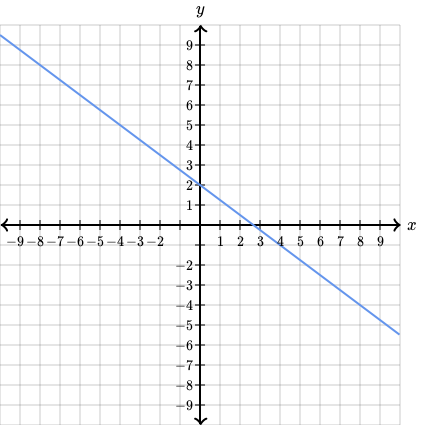
\includegraphics[scale=\shrinkfactor]{figures/12420e4e28e49d4985463bfbd43fcb1405cfb0d7.png}

\paragraph{Ans} 

\fbox{ $y=-\frac{3}{4}x+2$

}

 $y=-\frac{3}{4}x$

$y=\frac{3}{4}x+2$

$y=\frac{3}{4}x$



\paragraph{Hint 1}Let's find the rate of change of the graph, which is also what we call the *slope* of the graph. We need the exact coordinates of two points the graph passes through, so let's find two points whose values are integers. There are several points like this. We will use $(\red{0},\red{2})$ and $(\pink{8},\pink{-4})$.  
  

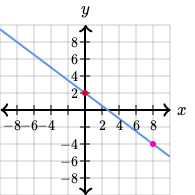
\includegraphics[scale=\shrinkfactor]{figures/2ab2ab7cc941094622dca436b2d08303f9e3c729.png}

\paragraph{Hint 2}The formula of the slope of the graph is **rise over run**, or in other words: (change in $y$)$/$(change in $x$).  
  
\begin{align*}\dfrac{(\pink{-4})-\red{2}}{\pink{8}-\red{0}}&=\dfrac{-6}{8}\\
&=-\dfrac{6}{8}\\
&=-\dfrac{\cancel{2}\cdot3}{\cancel{2}\cdot4}\\
&=-\dfrac{3}{4}
\end{align*}  
  
Therefore, the rate of change is $-\frac{3}{4}$.

\paragraph{Hint 3}There are *two* functions with this rate of change:  
$\quad y=-\dfrac{3}{4}x$  
and  
$\quad y=-\dfrac{3}{4}x+2$  
  
How do we decide which is the correct function?

\paragraph{Hint 4}Note that the first function represents a proportional relationship, and therefore its graph passes through the origin, meaning the point $(0,0)$. Our graph *doesn't* pass through the origin and therefore isn't described by the first function.

\paragraph{Hint 5}The only function that has the correct rate of change and doesn't describe a proportional relationship is:  
$\quad y=-\dfrac{3}{4}x+2$  
Therefore, this is the correct function.



\medskip
\noindent
\textbf{Tags:} {\footnotesize CC.8.F.B.4, SB.8.1.F.2.CR.1, Slope of a line.2}\\
\textbf{Version:} 962b8c35.. 2013-10-14
\smallskip\hrule





\section{\href{https://www.khanacademy.org/devadmin/content/items/xb48a795b}{xb48a795b}}

\noindent
Dulce the baker likes his bread sweet. For every $10$ grams of table salt he uses, he adds $25$ grams of sugar.
  
**Assuming the relationship is *proportional*, which function can represent the relationship between the amount of table salt in grams, $\text{T}$, and the amount of sugar in grams, $\text{S}$?**

\paragraph{Ans} 

\fbox{ $\text{S}=\frac{5}{2}\text{T}$

}

 $\text{S}=25+\frac{5}{2}\text{T}$

$\text{S}=\frac{10}{25}\text{T}$

$\text{S}=10+\frac{10}{25}\text{T}$



\paragraph{Hint 1}We know that for every $10$ grams of table salt he uses, Dulce adds $25$ grams of sugar. So how many grams of sugar will he add to $1$ gram of table salt?

\paragraph{Hint 2}\begin{align*}\dfrac{25}{10}&=\dfrac{\cancel{5}\cdot5}{\cancel{5}\cdot2}\\
&=\dfrac{5}{2}\end{align*}  
  
The rate of change is $\frac{5}{2}$.  
  
There are *two* functions with this rate of change:  
$\quad\text{S}=\dfrac{5}{2}\text{T}$  
and  
$\quad\text{S}=25+\dfrac{5}{2}\text{T}$  
  
How do we decide which is the correct function?

\paragraph{Hint 3}Remember that we are told the relationship is *proportional*. Since the second equation doesn't represent a proportional relationship, we must rule it out.

\paragraph{Hint 4}The only function with the correct rate of change that represents a proportional relationship is:  
$\quad\text{S}=\dfrac{5}{2}\text{T}$  
Therefore, this is the correct function.



\medskip
\noindent
\textbf{Tags:} {\footnotesize CC.8.F.B.4, SB.8.1.F.2.CR.1, Slope of a line.2}\\
\textbf{Version:} 571dce2c.. 2013-10-14
\smallskip\hrule





\section{\href{https://www.khanacademy.org/devadmin/content/items/xc27f0d7f}{xc27f0d7f}}

\noindent
**Determine which function corresponds to the following graph by finding the rate of change of the graph.**
  

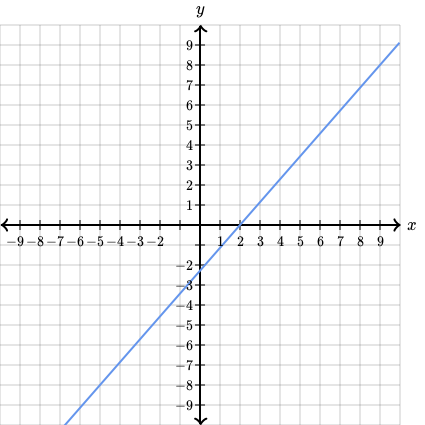
\includegraphics[scale=\shrinkfactor]{figures/81c06bf8c9102a6e969a4b60953e7dfa63955659.png}

\paragraph{Ans} 

\fbox{ $y=\frac{8}{7}x-2\frac{2}{7}$

}

 $y=2\frac{2}{7}-\frac{8}{7}x$

$y=-2\frac{2}{7}-\frac{7}{8}x$

$y=\frac{7}{8}x-2\frac{2}{7}$



\paragraph{Hint 1}Let's find the rate of change of the graph, which is also what we call the *slope* of the graph. We need the exact coordinates of two points the graph passes through, so let's find two points whose values are integers. There are several points like this. We will use $(\red{-5},\red{-8})$ and $(\pink{2},\pink{0})$.  
  

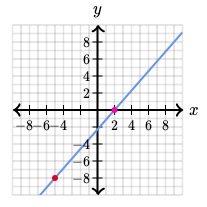
\includegraphics[scale=\shrinkfactor]{figures/0c3ea69fe77e9cb913abe45c623c249a6001a5fa.png}

\paragraph{Hint 2}The formula of the slope of the graph is **rise over run**, or in other words: (change in $y$)$/$(change in $x$).  
  
$\quad\dfrac{\pink{0}-(\red{-8})}{\pink{2}-(\red{-5})}=\dfrac{8}{7}$  
  
Therefore, the rate of change is $\frac{8}{7}$.

\paragraph{Hint 3}The only function that has the correct rate of change  is:  
$\quad y=\dfrac{8}{7}x-2\dfrac{2}{7}$  
Therefore, this is the correct function.



\medskip
\noindent
\textbf{Tags:} {\footnotesize CC.8.F.B.4, SB.8.1.F.2.CR.1, Slope of a line.2}\\
\textbf{Version:} 5229143d.. 2013-10-14
\smallskip\hrule





\section{\href{https://www.khanacademy.org/devadmin/content/items/xe0c136c7}{xe0c136c7}}

\noindent
**Determine which function corresponds to the following graph by finding the rate of change of the graph.**
  

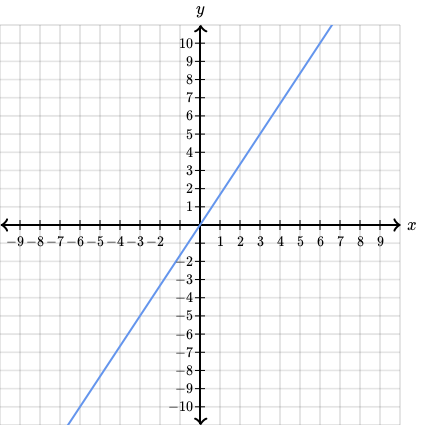
\includegraphics[scale=\shrinkfactor]{figures/5f4f69578da14d5190cd53b746a65d8bc074aa2a.png}

\paragraph{Ans} 

\fbox{ $y=\frac{5}{3}x$

}

 $y=\frac{5}{3}x+\frac{5}{3}$

$y=\frac{3}{5}x$

$y=\frac{3}{5}x+\frac{3}{5}$



\paragraph{Hint 1}Let's find the rate of change of the graph, which is also what we call the *slope* of the graph. We need the exact coordinates of two points the graph passes through, so let's find two points whose values are integers. There are several points like this. We will use $(\red{-6},\red{-10})$ and $(\pink{3},\pink{5})$.  
  

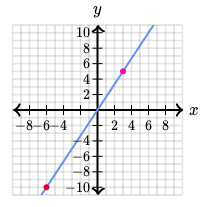
\includegraphics[scale=\shrinkfactor]{figures/b91bfa5d64aeeea1c1f10f7313db70b6b4715f46.png}

\paragraph{Hint 2}The formula of the slope of the graph is **rise over run**, or in other words: (change in $y$)$/$(change in $x$).  
  
\begin{align*}\dfrac{\pink{5}-(\red{-10})}{\pink{3}-(\red{-6})}&=\dfrac{15}{9}\\
&=\dfrac{\cancel{3}\cdot5}{\cancel{3}\cdot3}\\
&=\dfrac{5}{3}
\end{align*}  
  
Therefore, the rate of change is $\frac{5}{3}$.

\paragraph{Hint 3}There are *two* functions with this rate of change:  
$\quad y=\dfrac{5}{3}x$  
and  
$\quad y=\dfrac{5}{3}x+\dfrac{5}{3}$  
  
How do we decide which is the correct function?

\paragraph{Hint 4}Note that the second function doesn't represent a proportional relationship, and therefore its graph doesn't pass through the origin, meaning the point $(0,0)$. Our graph *passes* through the origin and therefore isn't described by the second function.

\paragraph{Hint 5}The only function that has the correct rate of change and describes a proportional relationship is:  
$\quad y=\dfrac{5}{3}x$  
Therefore, this is the correct function.



\medskip
\noindent
\textbf{Tags:} {\footnotesize CC.8.F.B.4, SB.8.1.F.2.CR.1, Slope of a line.2}\\
\textbf{Version:} 55de4674.. 2013-10-14
\smallskip\hrule





\section{\href{https://www.khanacademy.org/devadmin/content/items/xf7035987}{xf7035987}}

\noindent
"Simba" travel agency came out with a special offer for Mountain Kilimanjaro - pay as you climb!  
The table below describes the relationship between the altitude of the climb and the price to pay to get there.  
  
**Assuming the rate of change is constant, which function can represent the price paid for climbing, $\text{P}$, as a function of the altitude in meters, $\text{A}$?**  
  
Altitude (meters) | Price ($\$$)
:-:|:-:|:-:|
$3962$  (Shira Volcanic Cone) | $350$
$5149$ (Mawenzi Volcanic Cone)| $528.05$
$5895$ (Kibo Volcanic Cone)| $639.95$

\paragraph{Ans} 

$\text{P}=\frac{20}{3}\text{A}+350$

$\text{P}=639\frac{96}{100}-\frac{3}{20}\text{A}$

\fbox{ $\text{P}=-244\frac{3}{10}+\frac{3}{20}\text{A}$

}

 $\text{P}=-\frac{20}{3}\text{A}+3962$



\paragraph{Hint 1}The second row tells us that to get to an altitude of $\red{5149\text{ meters}}$, the price is $\red{\$528.05}$.  
The third row tells us that to get to an altitude of $\blue{5895\text{ meters}}$, the price is $\blue{\$639.95}$.  
  
$\quad\blue{5895}-\red{5149}=746$    
  
$\quad\blue{639.95}-\red{528.05}=111.90$  
  
Therefore, an increase of $746$ meters in altitude increases the price by $\$111.90$. Now let's find the increase in price for an increase of $1$ meter in altitude.

\paragraph{Hint 2}\begin{align*}\dfrac{111.90}{746}&=\dfrac{111.9\cdot10}{746\cdot10}\\
&=\dfrac{1119}{7460}\\
&=\dfrac{\cancel{373}\cdot3}{\cancel{373}\cdot20}\\
&=\dfrac{3}{20}\end{align*}  
  
So the rate of change is $\frac{3}{20}$.  
Note that what we did was like finding the slope of the line that passes through the points $(\red{5149}\text{ , }\red{528.05})$ and $(\blue{5895}\text{ , }\blue{639.95})$.

\paragraph{Hint 3}The only function with the above rate of change is:  
$\quad\text{P}=-244\dfrac{3}{10}+\dfrac{3}{20}\text{A}$  
Therefore, this is the correct function.



\medskip
\noindent
\textbf{Tags:} {\footnotesize CC.8.F.B.4, SB.8.1.F.2.CR.1, Slope of a line.2}\\
\textbf{Version:} d98cf7ad.. 2013-10-14
\smallskip\hrule





\section{\href{https://www.khanacademy.org/devadmin/content/items/x006df951}{x006df951}}

\noindent
Rachel is driving her truck from Boston to Chicago. Rachel drives $15$ kilometers every $10$ minutes.  
  
Consider the relationship between the time since Rachel started driving and the remaining distance to get to Chicago. We know the relationship has a constant rate of change.

**Which statement is correct?**

\paragraph{Ans} 

The relationship between time and remaining distance is proportional.

\fbox{ The remaining distance decreases by $45$ kilometers every $\frac{1}{2}$ hour that passes.

}

 Both statements are correct.

None of the statements is correct.



\paragraph{Hint 1}Let�s consider each statement separately, starting with "The relationship between time and remaining distance is proportional." Since the relationship is linear, both variables have to be $0$ together for it to be proportional. Do they?

\paragraph{Hint 2}No. At the beginning of the ride, when time is $0$ minutes, the distance is the *entire* distance from Boston to Chicago which is certainly not $0$. The statement is incorrect.  
  
Now let's consider "The remaining distance decreases by $45$ kilometers every $\frac{1}{2}$ hour that passes." $\frac{1}{2}$ hour is $30$ minutes, so the statement means that Rachel drives $45\text{ km}$ in $30$ minutes. Is that true?

\paragraph{Hint 3}We know that Rachel drives $15\text{ km}$ in $10$ minutes, so she drives a distance $3$ times as that in $30$ minutes, meaning $45\text{ km}$. Therefore, the statement is correct.

\paragraph{Hint 4}The only correct statement is "The remaining distance decreases by $45$ kilometers every $\frac{1}{2}$ hour that passes."



\medskip
\noindent
\textbf{Tags:} {\footnotesize CC.8.F.B.4, SB.8.1.F.2.CR.1, Slope of a line.3}\\
\textbf{Version:} 26074721.. 2013-10-15
\smallskip\hrule





\section{\href{https://www.khanacademy.org/devadmin/content/items/x06db4299febe19f4}{x06db4299febe19f4}}

\noindent
Isaac is filling up his suitcase with pants and socks. The following equation describes the relationship between the number of pants Isaac is packing, $\text{P}$, and the corresponding number of socks that fits in the suitcase, $\text{S}$.
  
$\quad\text{S}=28-\frac{7}{2}\text{P}$  
  
**Which statement is correct?**

\paragraph{Ans} 

\fbox{ When the number of pants decreases, the number of socks increases.

}

 If Isaac takes $7$ pants out of the suitcase, he makes room for $2$ more socks.

Both statements are correct.

None of the statements is correct.



\paragraph{Hint 1}Let�s consider each statement separately, starting with "When the number of pants decreases, the number of socks increases." This is equivalent to saying that the rate of change of the relationship is negative. Is it?

\paragraph{Hint 2}The rate of change is the number multiplied by $\text{P}$ in the equation, which is $-\frac{7}{2}$. The number is negative and therefore the statement is correct.  
  
Now let's consider "If Isaac takes $7$ pants out of the suitcase, he makes room for $2$ more socks." Let's use the rate of change to check the statement.

\paragraph{Hint 3}According to the rate of change, each pair of pants Isaac takes out leaves room for another $\frac{7}{2}$ socks. Therefore, taking out $7$ pants would leave room for:  
  
$\quad7\cdot\dfrac{7}{2}=\dfrac{49}{2}=24\dfrac{1}{2}$  
  
So the statement is incorrect.

\paragraph{Hint 4}The only correct statement is "When the number of pants decreases, the number of socks increases."



\medskip
\noindent
\textbf{Tags:} {\footnotesize CC.8.F.B.4, SB.8.1.F.2.CR.1, Slope of a line.3}\\
\textbf{Version:} 0cb728eb.. 2013-10-15
\smallskip\hrule





\section{\href{https://www.khanacademy.org/devadmin/content/items/x1582a380cef2e837}{x1582a380cef2e837}}

\noindent
Entrance to the paintball court with $4$ paint balls costs $\$2.20$ and entrance with $20$ balls costs $\$11$.  
  
Consider the relationship between the number of paint balls and the price of the ticket. We know the relationship has a constant rate of change.
  
**Which statement is correct?**

\paragraph{Ans} 

The slope of the graph of the relationship, where the $x$-axis represents number of paint balls, is undefined.

\fbox{ Entrance with $24$ balls costs $\$13.20$

}

 Both statements are correct.

None of the statements is correct.



\paragraph{Hint 1}Let�s consider each statement separately, starting with "The slope of the graph of the relationship, where the $x$-axis represents number of paint balls, is undefined." The relationship is linear, so its graph is a line. Can it be that the slope of this line is undefined?

\paragraph{Hint 2}An undefined slope means a vertical line, like in this example:  
  

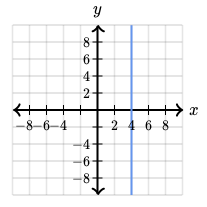
\includegraphics[scale=\shrinkfactor]{figures/1ac674b93f509bd69d4a7003be6a3a04d5ffc2a4.png}  
  
This means that $x$ has only one possible value. But we know that isn't true. So the statement is incorrect.  
  
Now let's consider "Entrance with $24$ balls costs $\$13.20$." Let's find the rate of change of the relationship, in order to check the statement.

\paragraph{Hint 3}Entrance with $\red{4\text{ balls}}$ costs $\red{\$2.20}$.  
Entrance with $\green{20\text{ balls}}$ costs $\green{\$11}$.  
  
The rate of change is the value of the ratio between the change in price and the change in number of balls:  
  
\begin{align*}\dfrac{\green{11}-\red{2.20}}{\green{20}-\red{4}}&=\dfrac{8.80}{16}\\
&=\dfrac{8.80\cdot10}{16\cdot10}\\
&=\dfrac{88}{160}\\
&=\dfrac{\cancel{8}\cdot11}{\cancel{8}\cdot20}\\
&=\dfrac{11}{20}\\
&=0.55
\end{align*}  
  
The rate of change is $\$0.55$ per paint ball. To find the price of a ticket with $24$ paint balls, we can add the price of $4$ balls to the price of a ticket with $20$ balls (which is $\$11$).  
Since each ball costs $\$0.55$, $4$ balls cost:  
  
$\quad0.55\cdot4=\$2.20$  
  
Therefore, a ticket with $24$ balls costs $11+2.20=\$13.20$. The statement is correct.  

\paragraph{Hint 4}The only correct statement is "Entrance with $24$ balls costs $\$13.20$."



\medskip
\noindent
\textbf{Tags:} {\footnotesize CC.8.F.B.4, SB.8.1.F.2.CR.1, Slope of a line.3}\\
\textbf{Version:} 523a4331.. 2013-10-15
\smallskip\hrule





\section{\href{https://www.khanacademy.org/devadmin/content/items/x170513858836f1aa}{x170513858836f1aa}}

\noindent
Rachel is driving her truck from Boston to Chicago. Rachel drives $15$ kilometers every $10$ minutes.  
  
Consider the relationship between the time since Rachel started driving and the remaining distance to get to Chicago. We know the relationship has a constant rate of change.

**Which statement is correct?**

\paragraph{Ans} 

\fbox{ The slope of the graph of the relationship between time and remaining distance is negative.

}

 When time increases by $1$ hour, the remaining distance increases by $90$ kilometers.

Both statements are correct.

None of the statements is correct.



\paragraph{Hint 1}Let�s consider each statement separately, starting with "The slope of the graph of the relationship between time and remaining distance is negative." We know the relationship is linear so its corresponding graph is a line.  
  
Suppose the $x$-axis represents the time that has passed. What happens to $y$, the remaining distance from Chicago, when $x$ increases?

\paragraph{Hint 2}$y$ *decreases*, since Rachel is always getting *closer* to Chicago. Therefore, the slope is indeed negative, and the statement is correct.  
  
Let's move on to the statement "When time increases by $1$ hour, the remaining distance increases by $90$ kilometers." Could this be true?

\paragraph{Hint 3}No. We already noted that the distance *decreases* when time increases. So the statement is incorrect.

\paragraph{Hint 4}The only correct statement is "The slope of the graph of the relationship between time and remaining distance is negative."



\medskip
\noindent
\textbf{Tags:} {\footnotesize CC.8.F.B.4, SB.8.1.F.2.CR.1, Slope of a line.3}\\
\textbf{Version:} 8a08c939.. 2013-10-15
\smallskip\hrule





\section{\href{https://www.khanacademy.org/devadmin/content/items/x2360c06637820bdf}{x2360c06637820bdf}}

\noindent
**Which statement regarding the graph below is correct?**  


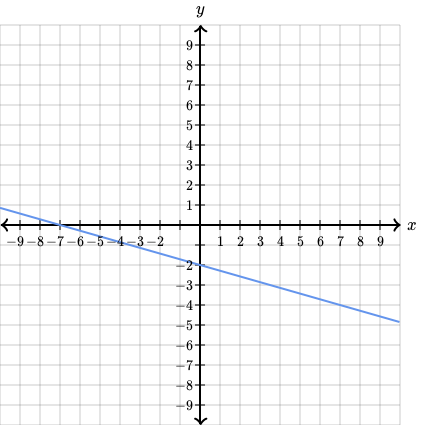
\includegraphics[scale=\shrinkfactor]{figures/42c898bd60f88a7c13c2a86541457cb5991e1dd1.png}

\paragraph{Ans} 

The slope of the graph is negative.

When $y$ increases by $1$, $x$ decreases by $3\frac{1}{2}$.

\fbox{ Both statements are correct.

}

 None of the statements is correct.



\paragraph{Hint 1}Let�s consider each statement separately, starting with "The slope of the graph is negative." We can see that the line is going down to the right, which means the slope is indeed negative (since $y$ *decreases* as $x$ increases). So the statement is correct.

\paragraph{Hint 2}Now let's consider "When $y$ increases by $1$, $x$ decreases by $3\frac{1}{2}$." Let's choose a point on the graph, increase $y$ by $1$, and see what happens to $x$. We need the exact values of the point that we choose, so let's take the point $(\red{0},\red{-2})$. If we increase $y$ by $1$ from $-2$ we get to $\pink{-1}$. What point on the graph corresponds to this value?

\paragraph{Hint 3}The corresponding point is $(\pink{-3\frac{1}{2}},\pink{-1})$:  
  

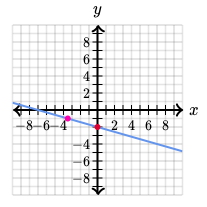
\includegraphics[scale=\shrinkfactor]{figures/f718ad269bdf66c6483dba95d9542f5aed9c3cae.png}  
  
The decrease in $x$ is indeed $3\frac{1}{2}$, so the statement is correct.

\paragraph{Hint 4}Both statements are correct.



\medskip
\noindent
\textbf{Tags:} {\footnotesize CC.8.F.B.4, SB.8.1.F.2.CR.1, Slope of a line.3}\\
\textbf{Version:} e0597331.. 2013-10-15
\smallskip\hrule





\section{\href{https://www.khanacademy.org/devadmin/content/items/x25261ad7}{x25261ad7}}

\noindent
Entrance to the paintball court costs $\$5$ and paint balls are paid for separately. A ticket for entrance with $5$ balls, for example, costs $\$8$.  
  
Consider the relationship between the number of paint balls and the price of the ticket. We know the relationship has a constant rate of change.
  
**Which statement is correct?**

\paragraph{Ans} 

The relationship is proportional.

\fbox{ When the number of balls increases by $11$, the price increases by $\$6.6$.

}

 Both statements are correct.

None of the statements is correct.



\paragraph{Hint 1}Let�s consider each statement separately, starting with "The relationship is proportional."  The relationship has a constant rate of change, but for it to be proportional, both variables have to be $0$ together. Are they?

\paragraph{Hint 2}We know that entrance without any balls costs $\$5$. This means that when the number of balls is $0$, the price isn't $0$. Therefore, the relationship isn't proportional, and the statement is incorrect.  
  
Now let's consider "When the number of balls increases by $11$, the price increases by $\$6.6$." This statement concerns the rate of change of the relationship. Let's find it.

\paragraph{Hint 3}Entrance with $\red{0\text{ balls}}$ costs $\red{\$5}$.  
Entrance with $\green{5\text{ balls}}$ costs $\green{\$8}$.  
  
The rate of change is the value of the ratio between the change in price and the change in number of balls:  
  
$\quad\dfrac{\green{8}-\red{5}}{\green{5}-\red{0}}=\dfrac{3}{5}=0.6$  
  
An addition of $1$ paint ball costs $\$0.60$.  
Therefore, an addition of $11$ balls costs:  
  
$\quad0.6\cdot11=\$6.6$  
  
The statement is correct.  

\paragraph{Hint 4}The only correct statement is:  
"When the number of balls increases by $11$, the price increases by $\$6.6$."



\medskip
\noindent
\textbf{Tags:} {\footnotesize CC.8.F.B.4, SB.8.1.F.2.CR.1, Slope of a line.3}\\
\textbf{Version:} 0496deaa.. 2013-10-15
\smallskip\hrule





\section{\href{https://www.khanacademy.org/devadmin/content/items/x385392b78ef3c652}{x385392b78ef3c652}}

\noindent
The table below describes the relationship between the number of minutes of mobile phone conversations and their price in some mobile carrier. The relationship has a constant rate of change.  
  
**Which statement is correct?**  
  
Conversations (minutes) | Price ($\$$)
:-:|:-:|:-:|
$50$ | $3.50$
$100$ | $5$
$200$ | $8$

\paragraph{Ans} 

The graph that describes this relationship passes through the origin, $(0,0)$.

$50$ minutes of conversation add $\$3.50$ to the price.

Both statements are correct.

\fbox{ None of the statements is correct.

}

 

\paragraph{Hint 1}Let�s consider each statement separately, starting with "$50$ minutes of conversation add $\$3.50$ to the price." This statement concerns the rate of change of the relationship. Let's find it.

\paragraph{Hint 2}$\red{100\text{ minutes}}$ of conversation cost $\red{\$5}$.  
$\green{200\text{ minutes}}$ of conversation cost $\green{\$8}$.  
  
The rate of change is the value of the ratio between the change in price and the change in length of conversations:  
  
$\quad\dfrac{\green{8}-\red{5}}{\green{200}-\red{100}}=\dfrac{3}{100}=0.03$  
  
The rate of change is $0.03$, which means each additional minute of conversation costs $\$0.03$.  Therefore, the price of $50$ additional minutes is:  
  
$\quad50\cdot0.03=\$1.50$  
  
So $50$ minutes add $\$1.50$ and not $\$3.50$. The statement is incorrect.  
  
Now let's consider "The graph that describes this relationship passes through the origin, $(0,0)$." This is equivalent to saying that both variables are $0$ together. Let's use what we've found so far to check the statement.

\paragraph{Hint 3}We know that the bill for $50$ minutes is $\$3.50$. We also know that a change of $50$ minutes brings a change of $\$1.50$ to the price.  
These changes can be negative as well. So if we subtract $\$1.50$ from $\$3.50$ we find that $0$ minutes cost $\$2$, and therefore the graph *doesn't* pass through the origin. The statement is incorrect.

\paragraph{Hint 4}None of the statements is correct.



\medskip
\noindent
\textbf{Tags:} {\footnotesize CC.8.F.B.4, SB.8.1.F.2.CR.1, Slope of a line.3}\\
\textbf{Version:} 67361a6f.. 2013-10-15
\smallskip\hrule





\section{\href{https://www.khanacademy.org/devadmin/content/items/x39250208}{x39250208}}

\noindent
**Which statement regarding the graph below is correct?**  


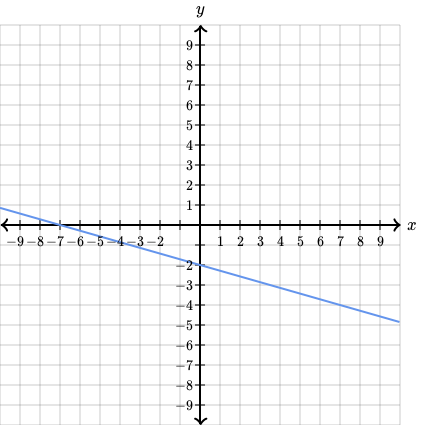
\includegraphics[scale=\shrinkfactor]{figures/42c898bd60f88a7c13c2a86541457cb5991e1dd1.png}

\paragraph{Ans} 

The relationship between $x$ and $y$ is proportional.

When $x$ decreases by $7$, $y$ decreases by $2$.

Both statements are correct.

\fbox{ None of the statements is correct.

}

 

\paragraph{Hint 1}Let�s consider each statement separately, starting with "The relationship between $x$ and $y$ is proportional." The graph of a proportional relationship is a line that passes through the origin, which is the point $(0,0)$. Our graph doesn't pass through the origin, so it doesn't describe a proportional relationship. The statement is incorrect.

\paragraph{Hint 2}Now let's consider "When $x$ decreases by $7$, $y$ decreases by $2$." This cannot be correct. We can see that the graph is going *down* to the right, which means the slope is *negative*. Therefore, when $x$ decreases, $y$ should *increase*.

\paragraph{Hint 3}None of the statements is correct.



\medskip
\noindent
\textbf{Tags:} {\footnotesize CC.8.F.B.4, SB.8.1.F.2.CR.1, Slope of a line.3}\\
\textbf{Version:} a468b433.. 2013-10-15
\smallskip\hrule





\section{\href{https://www.khanacademy.org/devadmin/content/items/x3cd1329e0073114a}{x3cd1329e0073114a}}

\noindent
The following formula describes the temperature in Fahrenheit degrees, $\text{F}$, as a function of the temperature in Celsius degrees, $\text{C}$:  
  
$\quad\text{F}=\frac{9}{5}\text{C}+32$  
  
**Which statement is correct?**

\paragraph{Ans} 

When the temperature increases in Celsius degrees, it also increases in Fahrenheit degrees.

If the temperature increased by $10^\circ\text{C}$, it means it increased by $18^\circ\text{F}$.

\fbox{ Both statements are correct.

}

 None of the statements is correct.



\paragraph{Hint 1}Let�s consider each statement separately, starting with "When the temperature increases in Celsius degrees, it also increases in Fahrenheit degrees." This is equivalent to saying that the rate of change of the relationship is positive. Is it?

\paragraph{Hint 2}The rate of change is the number multiplied by $\text{C}$ in the equation, which is $\frac{9}{5}$. The number is positive and therefore the statement is correct.  
  
Now let's consider "If the temperature increased by $10^\circ\text{C}$, it means it increased by $18^\circ\text{F}$." Let's use the rate of change to check this statement.

\paragraph{Hint 3}According to the rate of change, each time we increase $\text{C}$ by $1$, $\text{F}$ increases by $\frac{9}{5}$. Therefore, if we increase $\text{C}$ by $10$, $\text{F}$ increases by:  
  
$\quad10\cdot\dfrac{9}{5}=\dfrac{90}{5}=18$  
  
Therefore, the statement is correct.

\paragraph{Hint 4}Both statements are correct.



\medskip
\noindent
\textbf{Tags:} {\footnotesize CC.8.F.B.4, SB.8.1.F.2.CR.1, Slope of a line.3}\\
\textbf{Version:} cb339c00.. 2013-10-15
\smallskip\hrule





\section{\href{https://www.khanacademy.org/devadmin/content/items/x4a6cbb8a}{x4a6cbb8a}}

\noindent
**Which statement regarding the graph below is correct?**  


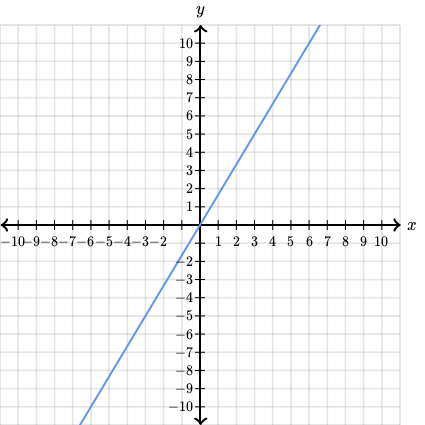
\includegraphics[scale=\shrinkfactor]{figures/fcd0daa4871157d97f75c78addc6cffab8213027.png}

\paragraph{Ans} 

The slope of the graph is negative.

\fbox{ When $x$ decreases by $6$, $y$ decreases by $10$.

}

 Both statements are correct.

None of the statements is correct.



\paragraph{Hint 1}Let�s consider each statement separately, starting with "The slope of the graph is negative." We can see that the line is going up to the right, which means the slope is *positive* (since $y$ *increases* when $x$ increases). So the statement is incorrect.

\paragraph{Hint 2}Now let's consider "When $x$ decreases by $6$, $y$ decreases by $10$." Let's choose a point on the graph, decrease $x$ by $6$ and see what happens to $y$. We need the exact values of the point that we choose, so let's take the point $(\red{0},\red{0})$. If we decrease $x$ by $6$ from $0$ we get to $\pink{-6}$. What point on the graph corresponds to this value?

\paragraph{Hint 3}The corresponding point is $(\pink{-6},\pink{-10})$:  
  

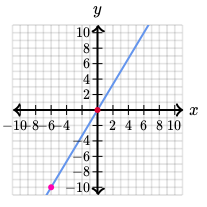
\includegraphics[scale=\shrinkfactor]{figures/0aef0d96f4ecf2237e931a0baefbdf70202b5574.png}  
  
The decrease in $y$ is indeed $10$, so the statement is correct.

\paragraph{Hint 4}The only correct statement is "When $x$ decreases by $6$, $y$ decreases by $10$."



\medskip
\noindent
\textbf{Tags:} {\footnotesize CC.8.F.B.4, SB.8.1.F.2.CR.1, Slope of a line.3}\\
\textbf{Version:} 5ba28300.. 2013-10-15
\smallskip\hrule





\section{\href{https://www.khanacademy.org/devadmin/content/items/x52ebdb32}{x52ebdb32}}

\noindent
The table below describes the relationship between the number of minutes of mobile phone conversations and their price in some mobile carrier. The relationship has a constant rate of change.  
  
**Which statement is correct?**  
  
Conversations (minutes) | Price ($\$$)
:-:|:-:|:-:|
$50$ | $3.50$
$100$ | $5$
$200$ | $8$

\paragraph{Ans} 

The slope of the graph of the relationship, where the $x$-axis represents the length of conversations, is less than $1$.

$\$0.75$ are worth another $25$ minutes of conversation.

\fbox{ Both statements are correct.

}

 None of the statements is correct.



\paragraph{Hint 1}Let�s consider each statement separately, starting with "$\$0.75$ are worth another $25$ minutes of conversation." This statement concerns the rate of change of the relationship. Let's find it.

\paragraph{Hint 2}$\red{100\text{ minutes}}$ of conversation cost $\red{\$5}$.  
$\green{200\text{ minutes}}$ of conversation cost $\green{\$8}$.  
  
The rate of change is the value of the ratio between the change in price and the change in length of conversations:  
  
$\quad\dfrac{\green{8}-\red{5}}{\green{200}-\red{100}}=\dfrac{3}{100}=0.03$  
  
The rate of change is $0.03$, which means each additional minute of conversation costs $\$0.03$.  Therefore, $25$ minutes of conversation are worth:  
  
$\quad25\cdot0.03=\$0.75$  
  
The statement is correct.  

\paragraph{Hint 3}Now let's consider "The slope of the graph of the relationship, where the $x$-axis represents the length of conversations, is less than $1$." The slope of the graph is equal to the rate of change we've found, which is $0.03$. Therefore, the slope is indeed less than $1$. The statement is correct.

\paragraph{Hint 4}Both statements are correct.



\medskip
\noindent
\textbf{Tags:} {\footnotesize CC.8.F.B.4, SB.8.1.F.2.CR.1, Slope of a line.3}\\
\textbf{Version:} ba5011fa.. 2013-10-15
\smallskip\hrule





\section{\href{https://www.khanacademy.org/devadmin/content/items/x5488daf25ffc29e6}{x5488daf25ffc29e6}}

\noindent
Entrance to the paintball court costs $\$5$ and paint balls are paid for separately. A ticket for entrance with $5$ balls, for example, costs $\$8$.  
  
Consider the relationship between the number of paint balls and the price of the ticket. We know the relationship has a constant rate of change.
  
**Which statement is correct?**

\paragraph{Ans} 

The graph of the relationship, where the $x$-axis represents the number of paint balls, has a slope of $\frac{5}{3}$.

Entrance with $10$ balls costs $\$16$.

Both statements are correct.

\fbox{ None of the statements is correct.

}

 

\paragraph{Hint 1}Let�s consider each statement separately, starting with "The graph of the relationship, where the $x$-axis represents the number of paint balls, has a slope of $\frac{5}{3}$." Let's find the slope of this graph.

\paragraph{Hint 2}Entrance with $\red{0\text{ balls}}$ costs $\red{\$5}$.  
Entrance with $\green{5\text{ balls}}$ costs $\green{\$8}$.  
  
The slope is the value of the ratio between the change in price and the change in number of balls:  
  
$\quad\dfrac{\green{8}-\red{5}}{\green{5}-\red{0}}=\dfrac{3}{5}=0.6$  
  
Therefore, the slope of the graph is $\frac{3}{5}$, which means an addition of $1$ paint ball costs $\$0.60$. According to the statement, the slope is $\frac{5}{3}$, so it's incorrect.  
  
Now let's consider "Entrance with $10$ balls costs $\$16$." Let's use what we've found so far to check the statement.

\paragraph{Hint 3}Entrance with $5$ paint balls costs $\$8$, and each addition of a single ball costs $\$0.6$. If we want to add $5$ balls to the ticket, we need to add:  
  
$\quad0.6\cdot5=\$3$  
  
Therefore, entrance with $10$ paint balls costs $\$11$ and not $\$16$. The statement is incorrect.

\paragraph{Hint 4}None of the statements is correct.



\medskip
\noindent
\textbf{Tags:} {\footnotesize CC.8.F.B.4, SB.8.1.F.2.CR.1, Slope of a line.3}\\
\textbf{Version:} 8d1db1a6.. 2013-10-15
\smallskip\hrule





\section{\href{https://www.khanacademy.org/devadmin/content/items/x6e8b68cd56f72fb4}{x6e8b68cd56f72fb4}}

\noindent
The table below describes the relationship between the number of minutes of mobile phone conversations and their price in some mobile carrier. The relationship has a constant rate of change.  
  
**Which statement is correct?**  
  
Conversations (minutes) | Price ($\$$)
:-:|:-:|:-:|
$30$ | $1.50$
$70$ | $3.50$
$100$ | $5$

\paragraph{Ans} 

The slope of the graph of the relationship, where the $x$-axis represents the length of conversations , is greater than $1$.

\fbox{ $25$ minutes of conversation add $\$1.25$ to the price.

}

 Both statements are correct.

None of the statements is correct.



\paragraph{Hint 1}Let�s consider each statement separately, starting with "$25$ minutes of conversation add $\$1.25$ to the price." This statement concerns the rate of change of the relationship. Let's find it.

\paragraph{Hint 2}$\red{30\text{ minutes}}$ of conversation cost $\red{\$1.50}$.  
$\green{70\text{ minutes}}$ of conversation cost $\green{\$3.50}$.  
  
The rate of change is the value of the ratio between the change in price and the change in length of conversations:  
  
\begin{align*}\dfrac{\green{3.50}-\red{1.50}}{\green{70}-\red{30}}&=\dfrac{2}{40}\\
&=\dfrac{\cancel{2}}{\cancel{2}\cdot20}\\
&=\dfrac{1}{20}\\
&=0.05
\end{align*}  
  
The rate of change is $0.05$, which means each additional minute of conversation costs $\$0.05$.  Now let's find the price of $25$ additional minutes.

\paragraph{Hint 3}$\quad25\cdot0.05=\$1.25$  
  
So the statement is correct.  
  
Now let's consider ""The slope of the graph of the relationship, where the $x$-axis represents the length of conversations , is greater than $1$." The slope of the graph is equal to the rate of change we've found, which is $0.05$. Therefore, the slope is *less* than $1$ and the statement is incorrect.

\paragraph{Hint 4}The only correct statement is "$25$ minutes of conversation add $\$1.25$ to the price."



\medskip
\noindent
\textbf{Tags:} {\footnotesize CC.8.F.B.4, SB.8.1.F.2.CR.1, Slope of a line.3}\\
\textbf{Version:} 1678ea9e.. 2013-10-15
\smallskip\hrule





\section{\href{https://www.khanacademy.org/devadmin/content/items/x6eb8a491da6157ec}{x6eb8a491da6157ec}}

\noindent
Dennis is riding his bicycle from his home to his office. Every $\frac{1}{4}$ hour Dennis rides $3$ miles.
  
Consider the relationship between the time since Dennis started riding and the distance he traveled in that time. We know the relationship has a constant rate of change.
  
**Which statement is correct?**

\paragraph{Ans} 

Dennis rides $\frac{3}{5}$ miles per minute.

It takes Dennis $3$ minutes to ride $1$ mile.

Both statements are correct.

\fbox{ None of the statements is correct.

}

 

\paragraph{Hint 1}Let's consider each statement separately, starting with "Dennis rides $\frac{3}{5}$ miles per minute." We know that Dennis rides $3$ miles in $\frac{1}{4}$ hour, which is $15$ minutes. How much does he ride in a single minute?

\paragraph{Hint 2}$\quad\dfrac{3}{15}=\dfrac{\cancel{3}}{\cancel{3}\cdot5}=\dfrac{1}{5}$  
  
So Dennis rides $\frac{1}{5}$ mile and not $\frac{3}{5}$. The statement is incorrect.
  
Now let's consider "It takes Dennis $3$ minutes to ride $1$ mile." Again, we know that Dennis rides $3$ miles in $15$ minutes. How long will it take him to ride a single mile?

\paragraph{Hint 3}$\quad\dfrac{15}{3}=5$  
  
So it takes Dennis $5$ minutes and not $3$ to ride a single mile, and the statement is incorrect.

\paragraph{Hint 4}None of the statements is correct.



\medskip
\noindent
\textbf{Tags:} {\footnotesize CC.8.F.B.4, SB.8.1.F.2.CR.1, Slope of a line.3}\\
\textbf{Version:} d9cb0659.. 2013-10-15
\smallskip\hrule





\section{\href{https://www.khanacademy.org/devadmin/content/items/x77f0fdd8}{x77f0fdd8}}

\noindent
Isaac is filling up his suitcase with pants and socks. The following equation describes the relationship between the number of pants Isaac is packing, $\text{P}$, and the corresponding number of socks that fits in the suitcase, $\text{S}$.
  
$\quad\text{S}=28-\frac{7}{2}\text{P}$  
  
**Which statement is correct?**

\paragraph{Ans} 

The graph of this equation passes through the origin.

\fbox{ If Isaac wants to add $14$ socks, he needs to take out $4$ pants.

}

 Both statements are correct.

None of the statements is correct.



\paragraph{Hint 1}Let�s consider each statement separately, starting with "The graph of this equation passes through the origin." This means that both variables have to be $0$ together. Let's substitute $0$ for $\text{P}$ in the equation.

\paragraph{Hint 2}$\quad\text{S}=28-\dfrac{7}{2}\cdot0=28-0=28$  
  
So when Isaac packs $0$ pants, he can fit $28$ socks. Therefore, the statement is incorrect.  
  
Now let's consider "If Isaac wants to add $14$ socks, he needs to take out $4$ pants." This statement concerns the rate of change of the relationship, so let's use it.

\paragraph{Hint 3}The rate of change is the number multiplied by $\text{P}$ in the equation, which is $-\frac{7}{2}$. This means that each pair of pants Isaac takes *out* leaves room for $\frac{7}{2}$ socks *more*. Therefore, taking out $4$ pants would leave room for:  
  
$\quad 4\cdot\dfrac{7}{2}=\dfrac{28}{2}=14$  
  
So the statement is correct.

\paragraph{Hint 4}The only correct statement is "If Isaac wants to add $14$ socks, he needs to take out $4$ pants."



\medskip
\noindent
\textbf{Tags:} {\footnotesize CC.8.F.B.4, SB.8.1.F.2.CR.1, Slope of a line.3}\\
\textbf{Version:} 8d98e86b.. 2013-10-15
\smallskip\hrule





\section{\href{https://www.khanacademy.org/devadmin/content/items/x7df3e4f9}{x7df3e4f9}}

\noindent
Dennis is riding his bicycle from his home to his office. Every $\frac{1}{4}$ hour Dennis rides $3$ miles.
  
Consider the relationship between the time since Dennis started riding and the distance he traveled in that time. We know the relationship has a constant rate of change.
  
**Which statement is correct?**

\paragraph{Ans} 

The relationship between time and distance traveled is proportional.

The slope of the graph of the relationship, where the $x$-axis represents the time in minutes , is less than $1$.

\fbox{ Both statements are correct.

}

 None of the statements is correct.



\paragraph{Hint 1}Let's consider each statement separately, starting with "The relationship between time and distance traveled is proportional." Since the relationship is linear, both variables need to be $0$ together for the relationship to be proportional. Do they?

\paragraph{Hint 2}At the beginning of the ride, time is $0$ minutes, and the distance traveled is $0$ miles. Therefore, the relationship is proportional, and the statement is correct.  
  
Now let's consider "The slope of the graph of the relationship, where the $x$-axis represents the time in minutes, is less than $1$." Since the relationship is linear, its corresponding graph is a line. Let's use the given information to check the statement.

\paragraph{Hint 3}We know that Dennis rides $3$ miles in $\frac{1}{4}$ hour, which is $15$ minutes.  
  
The change in $x$, time, is greater than the change in $y$, distance. Since the slope is the constant ratio between any change in $y$ and its corresponding change in $x$, the slope is indeed less than $1$. The statement is correct.

\paragraph{Hint 4}Both statements are correct.



\medskip
\noindent
\textbf{Tags:} {\footnotesize CC.8.F.B.4, SB.8.1.F.2.CR.1, Slope of a line.3}\\
\textbf{Version:} 74601c2c.. 2013-10-15
\smallskip\hrule





\section{\href{https://www.khanacademy.org/devadmin/content/items/x819030b668d06769}{x819030b668d06769}}

\noindent
**Which statement regarding the graph below is correct?**  


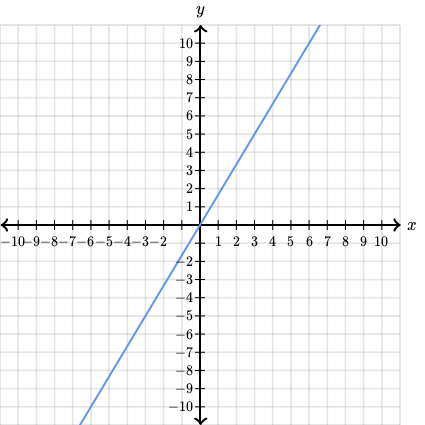
\includegraphics[scale=\shrinkfactor]{figures/fcd0daa4871157d97f75c78addc6cffab8213027.png}

\paragraph{Ans} 

\fbox{ The relationship between $x$ and $y$ is proportional.

}

 When $y$ increases by $3$, $x$ increases by $5$.

Both statements are correct.

None of the statements is correct.



\paragraph{Hint 1}Let�s consider each statement separately, starting with "The relationship between $x$ and $y$ is proportional." The graph of a proportional relationship is a line that passes through the origin, which is the point $(0,0)$. This is indeed the case with this graph, so the statement is correct.

\paragraph{Hint 2}Now let's consider "When $y$ increases by $3$, $x$ increases by $5$." Let's choose a point on the graph, increase $y$ by $3$ and see what happens to $x$. We need the exact values of the point that we choose, so let's take the point $(\red{0},\red{0})$. If we increase $y$ by $3$ from $0$ we get to $\green{3}$. What point on the graph corresponds to this value?

\paragraph{Hint 3}The corresponding point is $(\green{1.8},\green{3})$:  
  

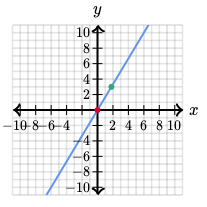
\includegraphics[scale=\shrinkfactor]{figures/b8b4541c15bbc7d5fc1508d6dd6a4a3dca600c8b.png}  
  
$x$ increased only by $1.8$, so the statement is incorrect.

\paragraph{Hint 4}The only correct statement is "The relationship between $x$ and $y$ is proportional."



\medskip
\noindent
\textbf{Tags:} {\footnotesize CC.8.F.B.4, SB.8.1.F.2.CR.1, Slope of a line.3}\\
\textbf{Version:} ca8fc0a2.. 2013-10-15
\smallskip\hrule





\section{\href{https://www.khanacademy.org/devadmin/content/items/x8f9d9f60}{x8f9d9f60}}

\noindent
The following formula describes the temperature in Fahrenheit degrees, $\text{F}$, as a function of the temperature in Celsius degrees, $\text{C}$:  
  
$\quad\text{F}=\frac{9}{5}\text{C}+32$  
  
**Which statement is correct?**

\paragraph{Ans} 

When the temperature is $0^\circ\text{C}$, it is also $0^\circ\text{F}$.

If the temperature decreased by $9^\circ\text{C}$, it means it decreased by $5^\circ\text{F}$.

Both statements are correct.

\fbox{ None of the statements is correct.

}

 

\paragraph{Hint 1}Let�s consider each statement separately, starting with "When the temperature is $0^\circ\text{C}$, it is also $0^\circ\text{F}$." Let's substitute $0$ for $\text{C}$ in the equation.

\paragraph{Hint 2}$\quad\text{F}=\dfrac{9}{5}\cdot0+32=32$  
  
This means that when the temperature is $0^\circ\text{C}$, it is $32^\circ\text{F}$ and not $0^\circ\text{F}$. The statement is incorrect.  
  
Now let's consider "If the temperature decreased by $9^\circ\text{C}$, it means it decreased by $5^\circ\text{F}$." Let's use the rate of change to check this statement.

\paragraph{Hint 3}The rate of change is the number multiplied by $\text{C}$ in the equation, which is $\frac{9}{5}$. This means that each time we decrease $\text{C}$ by $1$, $\text{F}$ decreases by $\frac{9}{5}$. Therefore, if we decrease $\text{C}$ by $9$, $\text{F}$ decreases by:  
  
$\quad9\cdot\dfrac{9}{5}=\dfrac{81}{5}=16\dfrac{1}{5}$  
  
Therefore, the statement is incorrect.

\paragraph{Hint 4}None of the statements is correct.



\medskip
\noindent
\textbf{Tags:} {\footnotesize CC.8.F.B.4, SB.8.1.F.2.CR.1, Slope of a line.3}\\
\textbf{Version:} e91c8340.. 2013-10-15
\smallskip\hrule





\section{\href{https://www.khanacademy.org/devadmin/content/items/x96433542}{x96433542}}

\noindent
Entrance to the paintball court with $4$ paint balls costs $\$2.20$ and entrance with $20$ balls costs $\$11$.  
  
Consider the relationship between the number of paint balls and the price of the ticket. We know the relationship has a constant rate of change.
  
**Which statement is correct?**

\paragraph{Ans} 

\fbox{ Entrance without any paint balls is free.

}

 An addition of $12$ balls increases the price by $\$5.50$.

Both statements are correct.

None of the statements is correct.



\paragraph{Hint 1}Let�s consider each statement separately, starting with "An addition of $12$ balls increases the price by $\$5.50$." This statement is about the rate of change of the relationship, so let's find it.

\paragraph{Hint 2}Entrance with $\red{4\text{ balls}}$ costs $\red{\$2.20}$.  
Entrance with $\green{20\text{ balls}}$ costs $\green{\$11}$.  
  
The rate of change is the value of the ratio between the change in price and the change in number of balls:  
  
\begin{align*}\dfrac{\green{11}-\red{2.20}}{\green{20}-\red{4}}&=\dfrac{8.80}{16}\\
&=\dfrac{8.80\cdot10}{16\cdot10}\\
&=\dfrac{88}{160}\\
&=\dfrac{\cancel{8}\cdot11}{\cancel{8}\cdot20}\\
&=\dfrac{11}{20}\\
&=0.55
\end{align*}  
  
Therefore, the rate of change is $\$0.55$ per paint ball. An addition of $12$ balls should cost $12$ times as that, which is $\$6.60$. So the statement isn't correct.  
  
Now let's consider "Entrance without any paint balls is free." Let's use what we've found so far to check the statement.

\paragraph{Hint 3}We know that entrance with $4$ paint balls costs $\$2.20$. We also know that each paint ball costs $\$0.55$, so $4$ balls cost:  
  
$\quad0.55\cdot4=\$2.20$  
  
If we subtract the price of $4$ balls from the price of a ticket with $4$ balls, we get $\$0$. This means that entrance without any paint balls is free. The statement is correct.

\paragraph{Hint 4}The only correct statement is "Entrance without any paint balls is free."



\medskip
\noindent
\textbf{Tags:} {\footnotesize CC.8.F.B.4, SB.8.1.F.2.CR.1, Slope of a line.3}\\
\textbf{Version:} 1105532e.. 2013-10-15
\smallskip\hrule





\section{\href{https://www.khanacademy.org/devadmin/content/items/xb585f6f6}{xb585f6f6}}

\noindent
The table below describes the relationship between the number of minutes of mobile phone conversations and their price in some mobile carrier. The relationship has a constant rate of change.  
  
**Which statement is correct?**  
  
Conversations (minutes) | Price ($\$$)
:-:|:-:|:-:|
$30$ | $1.50$
$70$ | $3.50$
$100$ | $5$

\paragraph{Ans} 

\fbox{ The relationship is proportional.

}

 $\$40$ are worth another $2$ minutes of conversation.

Both statements are correct.

None of the statements is correct.



\paragraph{Hint 1}Let�s consider each statement separately, starting with ""$\$40$ are worth another $2$ minutes of conversation." This statement concerns the rate of change of the relationship. Let's find it.

\paragraph{Hint 2}$\red{30\text{ minutes}}$ of conversation cost $\red{\$1.50}$.  
$\green{70\text{ minutes}}$ of conversation cost $\green{\$3.50}$.  
  
The rate of change is the value of the ratio between the change in price and the change in length of conversations:  
  
\begin{align*}\dfrac{\green{3.50}-\red{1.50}}{\green{70}-\red{30}}&=\dfrac{2}{40}\\
&=\dfrac{\cancel{2}}{\cancel{2}\cdot20}\\
&=\dfrac{1}{20}\\
&=0.05
\end{align*}  
  
The rate of change is $0.05$, which means each additional minute of conversation costs $\$0.05$. Therefore, $2$ minutes of conversation are worth $\$0.10$, and not $\$40$. The statement is incorrect.  
  
Now let's consider "The relationship is proportional." Since the rate of change is constant, both variables have to be $0$ together for the relationship to be proportional. Let's check if they do.

\paragraph{Hint 3}We know that a total of $30$ minutes costs $\$1.50$. We also know that each minute costs $\$0.05$. Let's find the change in price for a change of $30$ minutes in conversations:  
  
$\quad30\cdot0.05=\$1.50$  
  
if we reduce this sum from the bill for a total amount of $30$ minutes, we get $\$0$. Therefore, $0$ minutes cost $\$0$ and the relationship is proportional. The statement is correct.

\paragraph{Hint 4}The only correct statement is "The relationship is proportional."



\medskip
\noindent
\textbf{Tags:} {\footnotesize CC.8.F.B.4, SB.8.1.F.2.CR.1, Slope of a line.3}\\
\textbf{Version:} 0038cec0.. 2013-10-15
\smallskip\hrule



%%  Create a directory called 'figures' in latex dir and run the following command 
%  wget -N \
%    https://ka-perseus-graphie.s3.amazonaws.com/61dbf4e2b952dfe6759074d49f6b0f4f6d9f2564.png \
%    https://ka-perseus-graphie.s3.amazonaws.com/3d24a6acea488b6bce2e1425babe02a277549931.png \
%    https://ka-perseus-graphie.s3.amazonaws.com/12420e4e28e49d4985463bfbd43fcb1405cfb0d7.png \
%    https://ka-perseus-graphie.s3.amazonaws.com/2ab2ab7cc941094622dca436b2d08303f9e3c729.png \
%    https://ka-perseus-graphie.s3.amazonaws.com/81c06bf8c9102a6e969a4b60953e7dfa63955659.png \
%    https://ka-perseus-graphie.s3.amazonaws.com/0c3ea69fe77e9cb913abe45c623c249a6001a5fa.png \
%    https://ka-perseus-graphie.s3.amazonaws.com/5f4f69578da14d5190cd53b746a65d8bc074aa2a.png \
%    https://ka-perseus-graphie.s3.amazonaws.com/b91bfa5d64aeeea1c1f10f7313db70b6b4715f46.png \
%    https://ka-perseus-graphie.s3.amazonaws.com/1ac674b93f509bd69d4a7003be6a3a04d5ffc2a4.png \
%    https://ka-perseus-graphie.s3.amazonaws.com/42c898bd60f88a7c13c2a86541457cb5991e1dd1.png \
%    https://ka-perseus-graphie.s3.amazonaws.com/f718ad269bdf66c6483dba95d9542f5aed9c3cae.png \
%    https://ka-perseus-graphie.s3.amazonaws.com/fcd0daa4871157d97f75c78addc6cffab8213027.png \
%    https://ka-perseus-graphie.s3.amazonaws.com/0aef0d96f4ecf2237e931a0baefbdf70202b5574.png \
%    https://ka-perseus-graphie.s3.amazonaws.com/b8b4541c15bbc7d5fc1508d6dd6a4a3dca600c8b.png \


\end{document}
